\begin{figure*}[t]
\centering
\subfloat[Per-Role F1 by Disease\label{tab:confusion_counts}]{\parbox[t][2.9cm][t]{0.32\textwidth}{\centering\vspace*{0.3cm}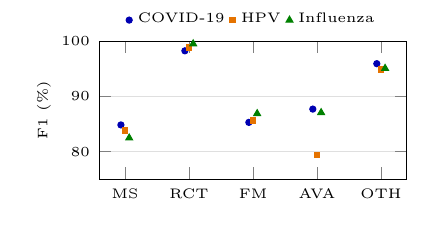
\begin{tikzpicture}\begin{axis}[ymajorgrids, grid style={gray!25}, tick label style={font=\tiny}, label style={font=\tiny}, title style={font=\tiny}, legend style={font=\tiny, draw=none, fill=none, at={(0.5,1.02)}, anchor=south}, legend columns=3, scale only axis, width=3.9cm, height=1.75cm, legend style={overlay}, ylabel shift=-3pt, symbolic x coords={MS,RCT,FM,AVA,OTH}, xtick={MS,RCT,FM,AVA,OTH}, ylabel={F1 (\%)}, ymin=75, ymax=100]\addplot[only marks,mark=*,mark size=1.1pt,color=blue!70!black,xshift=-1.5pt] coordinates {(MS,84.84)(RCT,98.28)(FM,85.30)(AVA,87.71)(OTH,95.95)};\addplot[only marks,mark=square*,mark size=1.0pt,color=orange!90!black] coordinates {(MS,83.78)(RCT,98.83)(FM,85.69)(AVA,79.38)(OTH,94.87)};\addplot[only marks,mark=triangle*,mark size=1.4pt,color=green!50!black,xshift=1.5pt] coordinates {(MS,82.47)(RCT,99.55)(FM,86.89)(AVA,87.07)(OTH,95.10)};\legend{COVID-19,HPV,Influenza}\end{axis}\end{tikzpicture}}}\hfill
\subfloat[Encoders by Disease\label{tab:standard_classifiers}]{\parbox[t][2.9cm][t]{0.32\textwidth}{\centering\vspace*{0.3cm}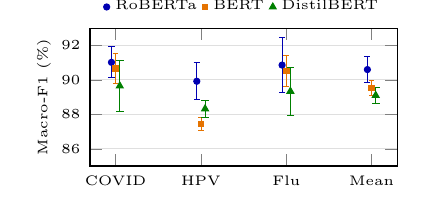
\begin{tikzpicture}\begin{axis}[ymajorgrids, grid style={gray!25}, tick label style={font=\tiny}, label style={font=\tiny}, title style={font=\tiny}, legend style={font=\tiny, draw=none, fill=none, at={(0.5,1.02)}, anchor=south}, legend columns=3, scale only axis, width=3.9cm, height=1.75cm, legend style={overlay}, ylabel shift=-3pt, symbolic x coords={COVID,HPV,Flu,Mean}, xtick={COVID,HPV,Flu,Mean}, ylabel={Macro-F1 (\%)}, ymin=85, ymax=93]\addplot[only marks,mark=*,mark size=1.1pt,color=blue!70!black,xshift=-1.5pt,error bars/.cd,y dir=both,y explicit,error bar style={line width=0.3pt}] coordinates {(COVID,91.02)+-(0,0.90)(HPV,89.92)+-(0,1.08)(Flu,90.86)+-(0,1.58)(Mean,90.60)+-(0,0.74)};\addplot[only marks,mark=square*,mark size=1.0pt,color=orange!90!black,error bars/.cd,y dir=both,y explicit,error bar style={line width=0.3pt}] coordinates {(COVID,90.66)+-(0,0.89)(HPV,87.43)+-(0,0.39)(Flu,90.52)+-(0,0.89)(Mean,89.54)+-(0,0.43)};\addplot[only marks,mark=triangle*,mark size=1.4pt,color=green!50!black,xshift=1.5pt,error bars/.cd,y dir=both,y explicit,error bar style={line width=0.3pt}] coordinates {(COVID,89.65)+-(0,1.49)(HPV,88.32)+-(0,0.48)(Flu,89.34)+-(0,1.39)(Mean,89.10)+-(0,0.45)};\legend{RoBERTa,BERT,DistilBERT}\end{axis}\end{tikzpicture}}}\hfill
\subfloat[Cross-Disease Transfer\label{tab:cross_disease_results}]{\parbox[t][2.9cm][t]{0.32\textwidth}{\centering\vspace*{0.3cm}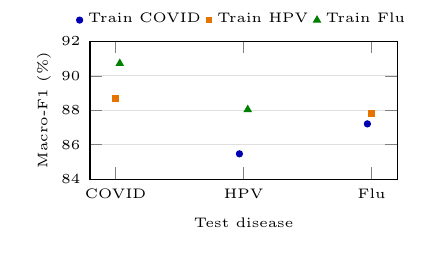
\begin{tikzpicture}\begin{axis}[ymajorgrids, grid style={gray!25}, tick label style={font=\tiny}, label style={font=\tiny}, title style={font=\tiny}, legend style={font=\tiny, draw=none, fill=none, at={(0.5,1.02)}, anchor=south}, legend columns=3, scale only axis, width=3.9cm, height=1.75cm, legend style={overlay}, ylabel shift=-3pt, symbolic x coords={COVID,HPV,Flu}, xtick={COVID,HPV,Flu}, xlabel={Test disease}, ylabel={Macro-F1 (\%)}, ymin=84, ymax=92]\addplot[only marks,mark=*,mark size=1.1pt,color=blue!70!black,xshift=-1.5pt] coordinates {(HPV,85.47)(Flu,87.21)};\addplot[only marks,mark=square*,mark size=1.0pt,color=orange!90!black] coordinates {(COVID,88.69)(Flu,87.82)};\addplot[only marks,mark=triangle*,mark size=1.4pt,color=green!50!black,xshift=1.5pt] coordinates {(COVID,90.72)(HPV,88.04)};\legend{Train COVID,Train HPV,Train Flu}\end{axis}\end{tikzpicture}}}
\caption{Supervised classification with fine-tuned encoders (means over three seeds and three disease folds). (a)~Per-role F1 for each disease (MS: \textit{Misinformation Spreader}; RCT: \textit{Religious Conspiracy Theorist}; FM: \textit{Fear Monger}; AVA: \textit{Anti-Vaccine Advocate}; OTH: \textit{Otherwise}). (b)~Macro-F1 of RoBERTa, BERT, and DistilBERT ($\pm$ standard deviation over seeds). (c)~Macro-F1 of RoBERTa trained on one disease and tested on another.}
\label{fig:supervised}
\vspace{-0.3cm}
\end{figure*}